\begin{appendices}

\chapter{Tabellen}
\begin{table}[h]
	\centering


	\resizebox{\columnwidth}{!}{%
		\begin{tabular}{|c|c|c|c|c|c|c|c|}
			\multicolumn{1}{c|}{} & \multicolumn{7}{c|}{Barkley}\\ 
			\hline \hline 
			\rule[-1ex]{0pt}{2.5ex} $a$ & 4 & 8 & 16 & 32 & 64 & 128 & 148\\ 
			\hline 
			\rule[-1ex]{0pt}{2.5ex} $b$ & 1 & 1 & 1 & 1 & 1 & 1 & 1 \\ 
			\hline 
			\rule[-1ex]{0pt}{3.5ex} $N$ & 400 & 400 & 50 & 200 & 400 & 200 & 50\\ 
			\hline 
			\rule[-1ex]{0pt}{3.5ex} $\rho(|\mathbf{W}|)$ & 0.8 & 0.5 & 0.5 & 1.5 & 1.5 & 3.0 & 0.8\\ 
			\hline 
			\rule[-1ex]{0pt}{3.5ex} $\alpha$ & 0.70 & 0.50 & 0.20 & 0.05 & 0.05 & 0.20 & 0.05 \\ 
			\hline 
			\rule[-1ex]{0pt}{3.5ex} $\epsilon$ & 0.2 & 0.2 & 0.1 & 0.2 & 0.2 & 0.2 & 0.1 \\ 
			\hline 
			\rule[-1ex]{0pt}{3.5ex} $\nu_{max}$ & $\num{1e-5}$ & $\num{1e-5}$ & $\num{1e-5}$ & $\num{1e-4}$ & $\num{1e-5}$ & $\num{1e-5}$ &  $\num{1e-5}$\\ 
			\hline 
			\rule[-1ex]{0pt}{3.5ex} $\lambda$ & $\num{5e-4}$ & $\num{5e-1}$ & $\num{5e-1}$ & $\num{5e+3}$ & $\num{5e+4}$ & $\num{5e+3}$ & $\num{5e-6}$\\ 		
			\hline 
			\rule[-1ex]{0pt}{2.5ex} Laufzeit [s] & 5 & 15 & 60 & 170 & 1922 & 3320 & 2970\\
			\hline 
			\rule[-1ex]{0pt}{2.5ex} \textbf{MSE} & \textbf{0.00005} & \textbf{0.00111} & \textbf{0.01447} & \textbf{0.09301} & \textbf{0.13093} & \textbf{0.15106} & \textbf{0.18380}\\ 
			\hline 
			\rule[-1ex]{0pt}{2.5ex} \textbf{NRMSE} & \textbf{0.0121} & \textbf{0.0801} & \textbf{0.3386} & \textbf{0.7398} & \textbf{0.9438} & \textbf{1.0098} & \textbf{1.1049} \\ 
			\hline 
		\end{tabular} 
	}
	
	\vspace{0.75cm}

	\centering
	
	\resizebox{\columnwidth}{!}{%
		\begin{tabular}{|c|c|c|c|c|c|c|c|}
			\multicolumn{1}{c|}{} & \multicolumn{7}{c|}{Mitchell-Schaeffer}\\ 
			\hline \hline 
			\rule[-1ex]{0pt}{2.5ex} $a$ & 4 & 8 & 16 & 32 & 64 & 128 & 148\\ 
			\hline 
			\rule[-1ex]{0pt}{2.5ex} $b$ & 1 & 1 & 1 & 1 & 1 & 1 & 1 \\ 
			\hline 
			\rule[-1ex]{0pt}{3.5ex} $N$ & 400 & 50 & 200 & 50 & 400 & 200 & 200\\ 
			\hline 
			\rule[-1ex]{0pt}{3.5ex} $\rho(|\mathbf{W}|)$ & 1.5 & 3.0 & 3.0 & 0.8 & 3.0 & 3.0 & 3.0\\ 
			\hline 
			\rule[-1ex]{0pt}{3.5ex} $\alpha$ & 0.95 & 0.50 & 0.05 & 0.95 & 0.20 & 0.05 & 0.05 \\ 
			\hline 
			\rule[-1ex]{0pt}{3.5ex} $\epsilon$ & 0.1 & 0.1 & 0.2 & 0.1 & 0.1 & 0.1 & 0.2 \\ 
			\hline 
			\rule[-1ex]{0pt}{3.5ex} $\nu_{max}$ & $\num{1e-4}$ & $\num{1e-5}$ & $\num{1e-5}$ & $\num{1e-5}$ & $\num{1e-4}$ & $\num{1e-5}$ &  $\num{1e-5}$\\ 
			\hline 
			\rule[-1ex]{0pt}{3.5ex} $\lambda$ & $\num{5e-0}$ & $\num{5e-2}$ & $\num{5e-1}$ & $\num{5e+3}$ & $\num{5e+3}$ & $\num{5e+4}$ & $\num{5e+4}$\\ 		
			\hline 
			\rule[-1ex]{0pt}{2.5ex} Laufzeit [s] & 3 & 9 & 27 & 121 & 548 & 3322 & 3021\\
			\hline 
			\rule[-1ex]{0pt}{2.5ex} \textbf{MSE} & \textbf{0.00023} & \textbf{0.00177} & \textbf{0.02969} & \textbf{0.05061} & \textbf{0.06330} & \textbf{0.06842} & \textbf{0.06761}\\ 
			\hline 
			\rule[-1ex]{0pt}{2.5ex} \textbf{NRMSE} & \textbf{0.0661} & \textbf{0.1704} & \textbf{0.6703} & \textbf{0.8861} & \textbf{0.9775} & \textbf{1.0166} & \textbf{1.0049} \\ 
			\hline 
		\end{tabular} 
	}

	\caption{Vollständige Auflistung der gefundenen Hyperparameter der \textsc{ESN}s für das \textit{Barkley}-Modell (oben) und das \textit{Mitchell-Schaeffer}-Modell (unten) für verschiedene Größen $a$ des vorherzusagenden Bereichs, welche zu den geringsten Fehlern führen. Zudem sind die benötigte Laufzeit und die erreichten Fehler angeführt.}
\label{tab:apx_inner_cross_esn_results}
\end{table}

\chapter{Abbildungen}

\begin{figure}[h]
	\centering
	\begin{subfigure}{.5\textwidth}
		\centering
		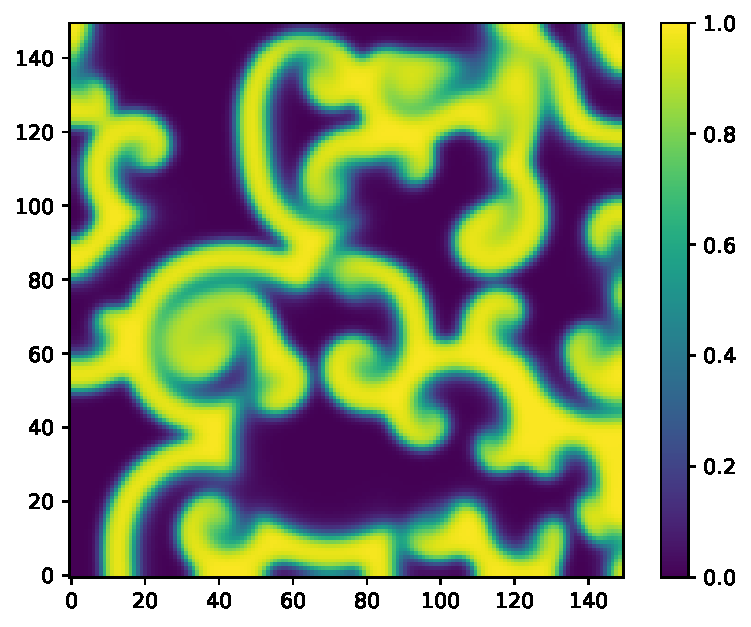
\includegraphics[height=2.5in]{figures/results/dynamics/barkley_0.pdf}
		\setcapmargin[1cm]{0.5cm}
		\caption{Erregung für $n=0$}
	\end{subfigure}%
	\begin{subfigure}{.5\textwidth}
		\centering
		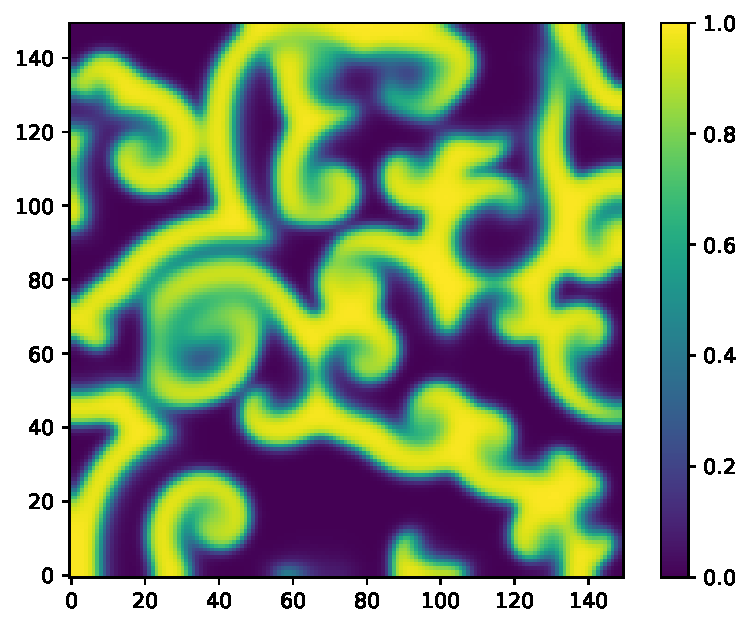
\includegraphics[height=2.5in]{figures/results/dynamics/barkley_50.pdf}
		\setcapmargin[1cm]{0.5cm}
		\caption{Erregung für $n=50$}
	\end{subfigure}
	\begin{subfigure}{.5\textwidth}
		\centering
		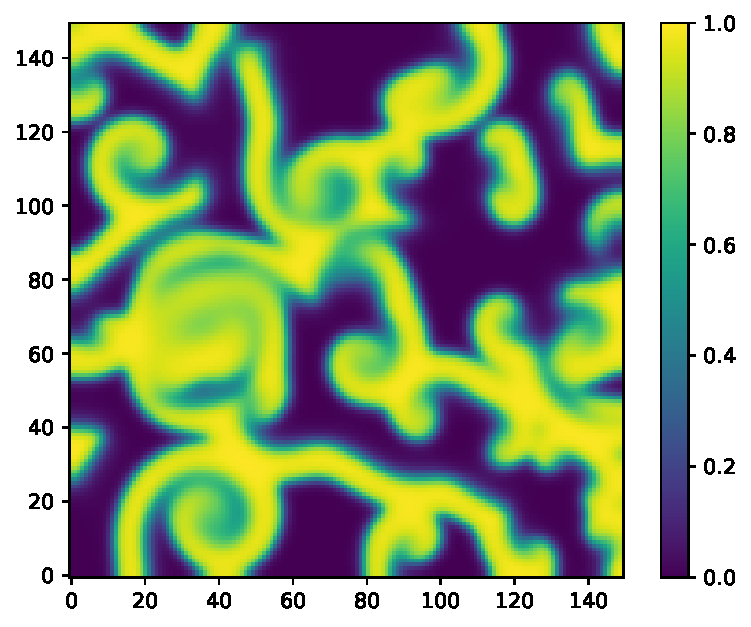
\includegraphics[height=2.5in]{figures/results/dynamics/barkley_100.pdf}
		\setcapmargin[1cm]{0.5cm}
		\caption{Erregung für $n=100$}
	\end{subfigure}%
	\begin{subfigure}{.5\textwidth}
		\centering
		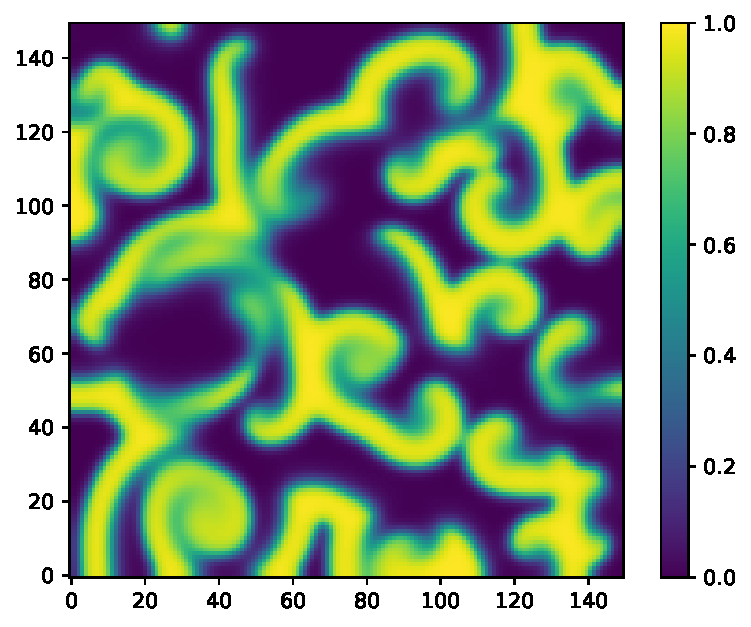
\includegraphics[height=2.5in]{figures/results/dynamics/barkley_150.pdf}
		\setcapmargin[1cm]{0.5cm}
		\caption{Erregung für $n=150$}
	\end{subfigure}
	\caption{Graphische Darstellung der zeitlichen Entwicklung der $u$-Variable des \textit{Barkley}-Modells. Im Uhrzeigersinn sind die Felder der $u$-Variable für die Zeitpunkte $t=0,\, 50,\, 100,\, 150$ des Evaluationsdatensatzes dargestellt.}
	\label{fig:apx_barkley_evolution}
\end{figure} 

\begin{figure}[h]
	\centering
	\begin{subfigure}{.5\textwidth}
		\centering
		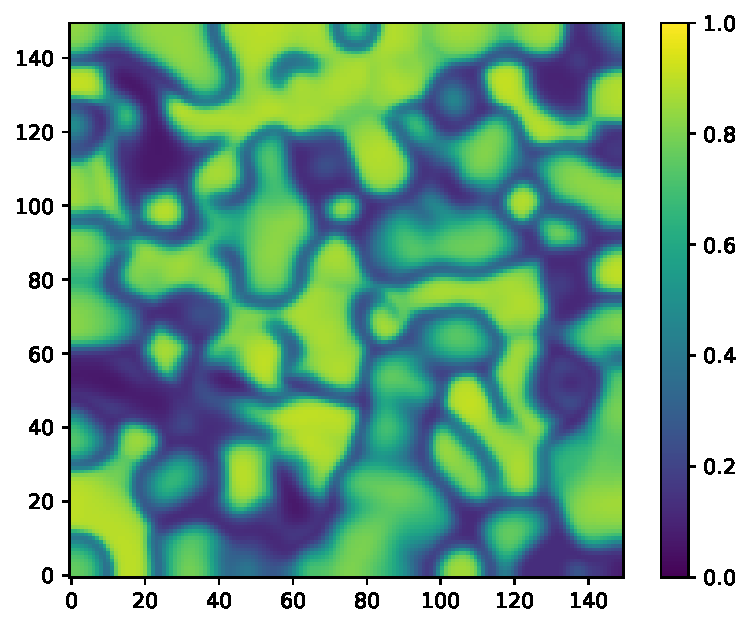
\includegraphics[height=2.5in]{figures/results/dynamics/mitchell_0.pdf}
		\setcapmargin[1cm]{0.5cm}
		\caption{Erregung für $n=0$}
	\end{subfigure}%
	\begin{subfigure}{.5\textwidth}
		\centering
		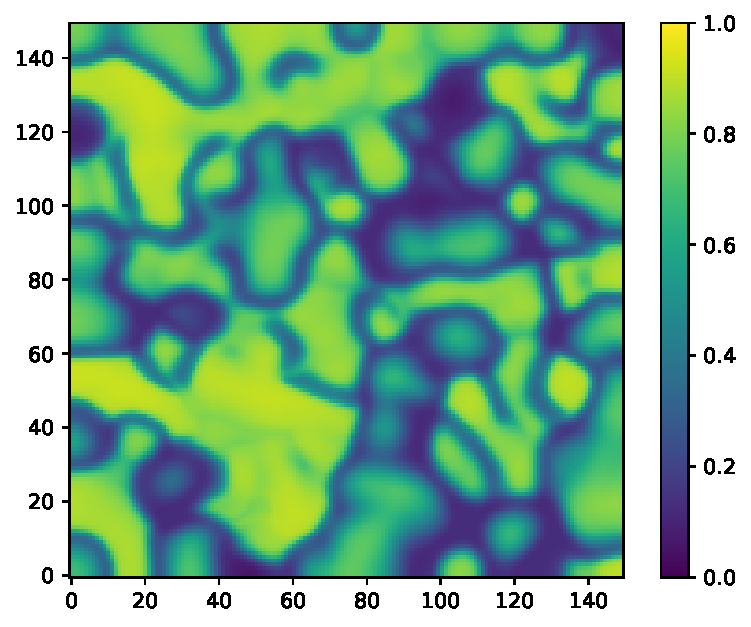
\includegraphics[height=2.5in]{figures/results/dynamics/mitchell_50.pdf}
		\setcapmargin[1cm]{0.5cm}
		\caption{Erregung für $n=50$}
	\end{subfigure}
	\begin{subfigure}{.5\textwidth}
		\centering
		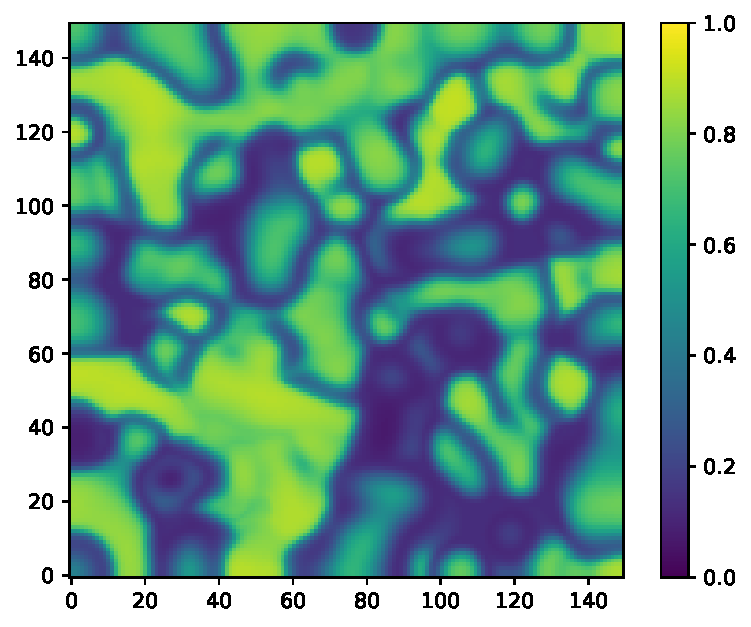
\includegraphics[height=2.5in]{figures/results/dynamics/mitchell_100.pdf}
		\setcapmargin[1cm]{0.5cm}
		\caption{Erregung für $n=100$}
	\end{subfigure}%
	\begin{subfigure}{.5\textwidth}
		\centering
		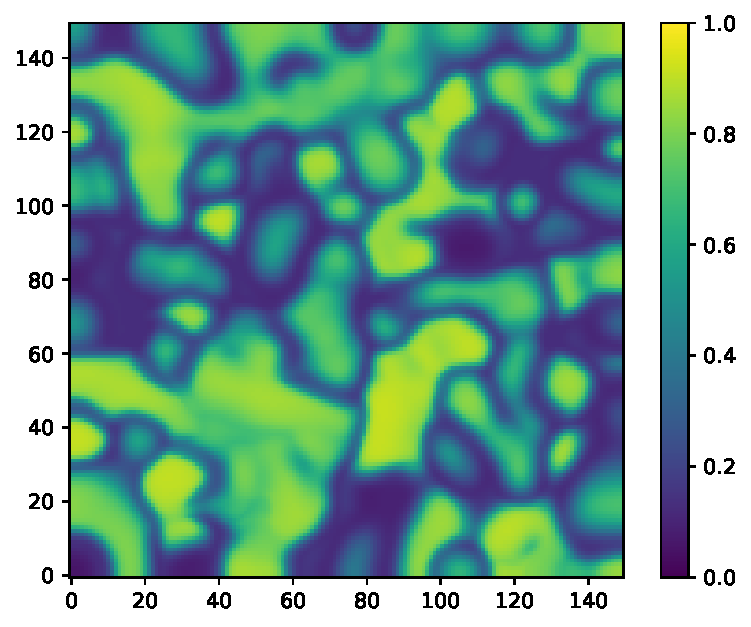
\includegraphics[height=2.5in]{figures/results/dynamics/mitchell_150.pdf}
		\setcapmargin[1cm]{0.5cm}
		\caption{Erregung für $n=150$}
	\end{subfigure}
	\caption{Graphische Darstellung der zeitlichen Entwicklung der $u$-Variable des \textit{Mitchell-Schaeffer}-Modells. Im Uhrzeigersinn sind die Felder der $v$-Variable für die Zeitpunkte $n=0,\, 50,\, 100,\, 150$ des Evaluationsdatensatzes dargestellt.}
	\label{fig:apx_mitchell_evolution}
\end{figure} 

\begin{figure}[h]
	\centering
	\begin{subfigure}{.5\textwidth}
		\centering
		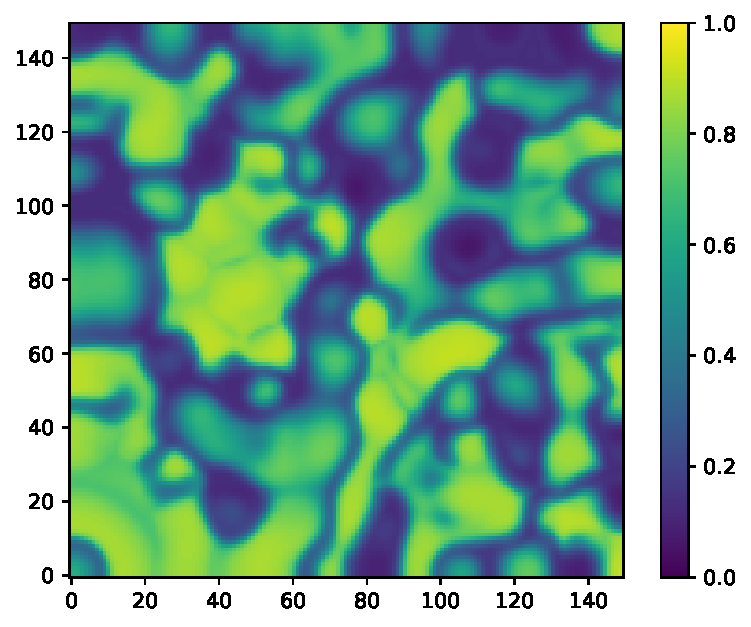
\includegraphics[height=2.5in]{figures/results/inner_cross_prediction/mitchell_v_inner_original.pdf}
		\setcapmargin[1cm]{0.5cm}
		\caption{Echte Erregung des Modells}
	\end{subfigure}%
	\begin{subfigure}{.5\textwidth}
		\centering
		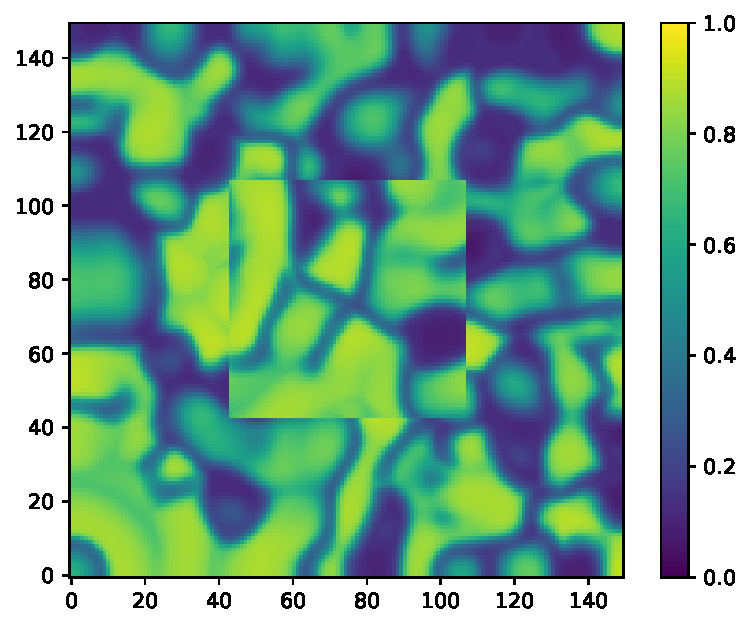
\includegraphics[height=2.5in]{figures/results/inner_cross_prediction/mitchell_v_inner_nn.pdf}
		\setcapmargin[1cm]{0.5cm}
  		\caption{Vorhersage des \textsc{NN}-Ansatzes}
	\end{subfigure}
	\begin{subfigure}{.5\textwidth}
		\centering
		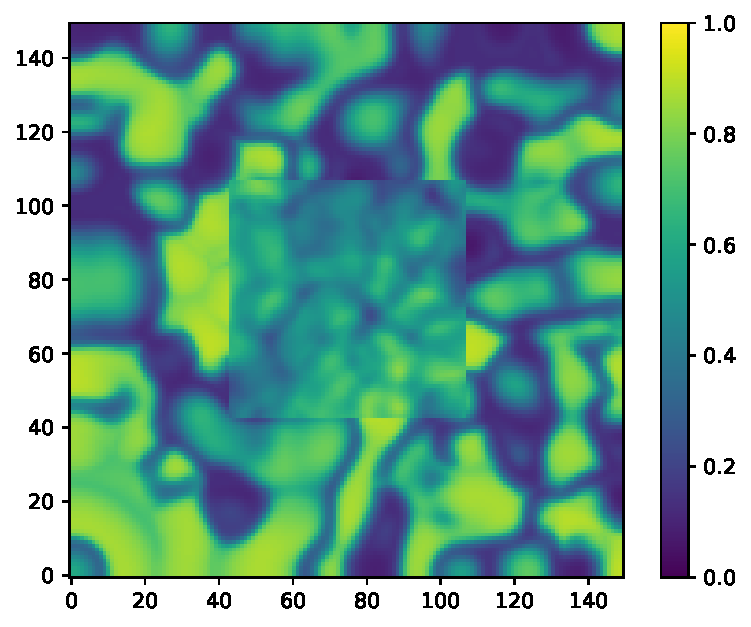
\includegraphics[height=2.5in]{figures/results/inner_cross_prediction/mitchell_v_inner_rbf.pdf}
		\setcapmargin[1cm]{0.5cm}
  		\caption{Vorhersage des \textsc{RBF}-Ansatzes}
	\end{subfigure}%
	\begin{subfigure}{.5\textwidth}
		\centering
		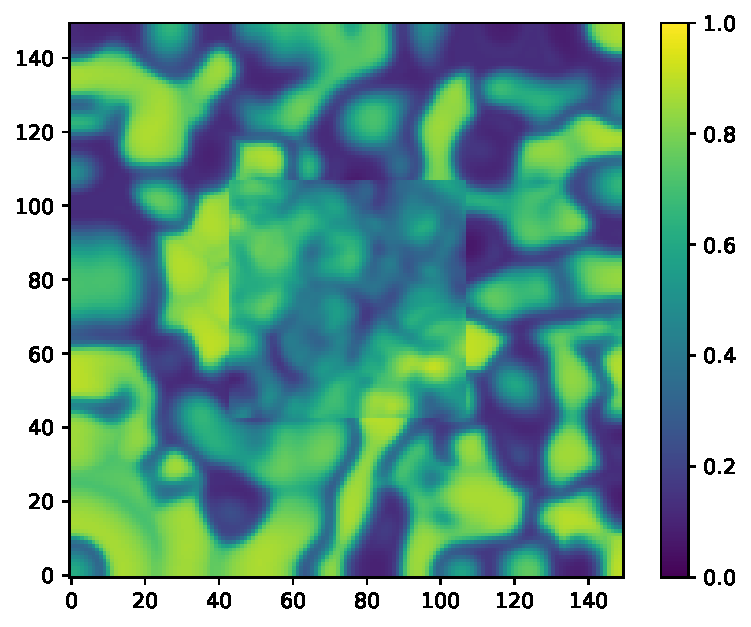
\includegraphics[height=2.5in]{figures/results/inner_cross_prediction/mitchell_v_inner_esn.pdf}
		\setcapmargin[1cm]{0.5cm}
  		\caption{Vorhersage des \textsc{ESN}}
	\end{subfigure}
	\caption{Graphische Darstellung der $v$-Variable des \textit{Mitchell-Schaeffer}-Modells für den $1000$. Zeitschritt des Evaluationsdatensatzes. Oben links ist das tatsächliche Feld des Modells zu sehen. Danach folgenden im Uhrzeigersinn die Vorhersagen des \textsc{NN}-Ansatzes, des \textsc{RBF}-Ansatzes und des \textsc{ESN}.}
	\label{fig:apx_inner_cross_mitchell_result}
\end{figure} 

\end{appendices}